\documentclass[12pt]{beamer}\usepackage[]{graphicx}\usepackage[]{color}
%% maxwidth is the original width if it is less than linewidth
%% otherwise use linewidth (to make sure the graphics do not exceed the margin)
\makeatletter
\def\maxwidth{ %
  \ifdim\Gin@nat@width>\linewidth
    \linewidth
  \else
    \Gin@nat@width
  \fi
}
\makeatother

\definecolor{fgcolor}{rgb}{0.345, 0.345, 0.345}
\newcommand{\hlnum}[1]{\textcolor[rgb]{0.686,0.059,0.569}{#1}}%
\newcommand{\hlstr}[1]{\textcolor[rgb]{0.192,0.494,0.8}{#1}}%
\newcommand{\hlcom}[1]{\textcolor[rgb]{0.678,0.584,0.686}{\textit{#1}}}%
\newcommand{\hlopt}[1]{\textcolor[rgb]{0,0,0}{#1}}%
\newcommand{\hlstd}[1]{\textcolor[rgb]{0.345,0.345,0.345}{#1}}%
\newcommand{\hlkwa}[1]{\textcolor[rgb]{0.161,0.373,0.58}{\textbf{#1}}}%
\newcommand{\hlkwb}[1]{\textcolor[rgb]{0.69,0.353,0.396}{#1}}%
\newcommand{\hlkwc}[1]{\textcolor[rgb]{0.333,0.667,0.333}{#1}}%
\newcommand{\hlkwd}[1]{\textcolor[rgb]{0.737,0.353,0.396}{\textbf{#1}}}%
\let\hlipl\hlkwb

\usepackage{framed}
\makeatletter
\newenvironment{kframe}{%
 \def\at@end@of@kframe{}%
 \ifinner\ifhmode%
  \def\at@end@of@kframe{\end{minipage}}%
  \begin{minipage}{\columnwidth}%
 \fi\fi%
 \def\FrameCommand##1{\hskip\@totalleftmargin \hskip-\fboxsep
 \colorbox{shadecolor}{##1}\hskip-\fboxsep
     % There is no \\@totalrightmargin, so:
     \hskip-\linewidth \hskip-\@totalleftmargin \hskip\columnwidth}%
 \MakeFramed {\advance\hsize-\width
   \@totalleftmargin\z@ \linewidth\hsize
   \@setminipage}}%
 {\par\unskip\endMakeFramed%
 \at@end@of@kframe}
\makeatother

\definecolor{shadecolor}{rgb}{.97, .97, .97}
\definecolor{messagecolor}{rgb}{0, 0, 0}
\definecolor{warningcolor}{rgb}{1, 0, 1}
\definecolor{errorcolor}{rgb}{1, 0, 0}
\newenvironment{knitrout}{}{} % an empty environment to be redefined in TeX

\usepackage{alltt}
\usepackage{graphicx}
\usepackage{tikz}
\setbeameroption{hide notes}
\setbeamertemplate{note page}[plain]
\usepackage{listings}

% do not include "../" so Makefile does not crash
% get rid of junk
\usetheme{default}
\usefonttheme[onlymath]{serif}
\beamertemplatenavigationsymbolsempty
\hypersetup{pdfpagemode=UseNone} % don't show bookmarks on initial view

% named colors
\definecolor{offwhite}{RGB}{255,250,240}
\definecolor{gray}{RGB}{155,155,155}

\ifx\notescolors\undefined % slides

  \definecolor{foreground}{RGB}{80,80,80}
  \definecolor{background}{RGB}{255,255,255}
  \definecolor{title}{RGB}{255,199,0}
  \definecolor{subtitle}{RGB}{89,132,212}
  \definecolor{hilit}{RGB}{248,117,79}
  \definecolor{vhilit}{RGB}{255,111,207}
  \definecolor{lolit}{RGB}{200,200,200}
  \definecolor{lit}{RGB}{255,199,0}
  \definecolor{mdlit}{RGB}{89,132,212}
  \definecolor{link}{RGB}{248,117,79}

\else % notes
  \definecolor{background}{RGB}{255,255,255}
  \definecolor{foreground}{RGB}{24,24,24}
  \definecolor{title}{RGB}{27,94,134}
  \definecolor{subtitle}{RGB}{22,175,124}
  \definecolor{hilit}{RGB}{122,0,128}
  \definecolor{vhilit}{RGB}{255,0,128}
  \definecolor{lolit}{RGB}{95,95,95}
\fi
\definecolor{nhilit}{RGB}{128,0,128}  % hilit color in notes
\definecolor{nvhilit}{RGB}{255,0,128} % vhilit for notes

\newcommand{\hilit}{\color{hilit}}
\newcommand{\vhilit}{\color{vhilit}}
\newcommand{\nhilit}{\color{nhilit}}
\newcommand{\nvhilit}{\color{nvhilit}}
\newcommand{\lit}{\color{lit}}
\newcommand{\mdlit}{\color{mdlit}}
\newcommand{\lolit}{\color{lolit}}

% use those colors
\setbeamercolor{titlelike}{fg=title}
\setbeamercolor{subtitle}{fg=subtitle}
\setbeamercolor{frametitle}{fg=gray}
\setbeamercolor{structure}{fg=subtitle}
\setbeamercolor{institute}{fg=lolit}
\setbeamercolor{normal text}{fg=foreground,bg=background}
%\setbeamercolor{item}{fg=foreground} % color of bullets
%\setbeamercolor{subitem}{fg=hilit}
%\setbeamercolor{itemize/enumerate subbody}{fg=lolit}
\setbeamertemplate{itemize subitem}{{\textendash}}
\setbeamerfont{itemize/enumerate subbody}{size=\footnotesize}
\setbeamerfont{itemize/enumerate subitem}{size=\footnotesize}

% center title of slides
\setbeamertemplate{blocks}[rounded]
\setbeamertemplate{frametitle}[default][center]
% margins
\setbeamersize{text margin left=25pt,text margin right=25pt}

% page number
\setbeamertemplate{footline}{%
    \raisebox{5pt}{\makebox[\paperwidth]{\hfill\makebox[20pt]{\lolit
          \scriptsize\insertframenumber}}}\hspace*{5pt}}

% add a bit of space at the top of the notes page
\addtobeamertemplate{note page}{\setlength{\parskip}{12pt}}

% default link color
\hypersetup{colorlinks, urlcolor={link}}

\ifx\notescolors\undefined % slides
  % set up listing environment
  \lstset{language=bash,
          basicstyle=\ttfamily\scriptsize,
          frame=single,
          commentstyle=,
          backgroundcolor=\color{darkgray},
          showspaces=false,
          showstringspaces=false
          }
\else % notes
  \lstset{language=bash,
          basicstyle=\ttfamily\scriptsize,
          frame=single,
          commentstyle=,
          backgroundcolor=\color{offwhite},
          showspaces=false,
          showstringspaces=false
          }
\fi

% a few macros
\newcommand{\code}[1]{\texttt{#1}}
\newcommand{\hicode}[1]{{\hilit \texttt{#1}}}
\newcommand{\bb}[1]{\begin{block}{#1}}
\newcommand{\eb}{\end{block}}
\newcommand{\bi}{\begin{itemize}}
%\newcommand{\bbi}{\vspace{24pt} \begin{itemize} \itemsep8pt}
\newcommand{\bbi}{\vspace{4pt} \begin{itemize} \itemsep8pt}
\newcommand{\ei}{\end{itemize}}
\newcommand{\bv}{\begin{verbatim}}
\newcommand{\ev}{\end{verbatim}}
\newcommand{\ig}{\includegraphics}
\newcommand{\subt}[1]{{\footnotesize \color{subtitle} {#1}}}
\newcommand{\ttsm}{\tt \small}
\newcommand{\ttfn}{\tt \footnotesize}
\newcommand{\figh}[2]{\centerline{\includegraphics[height=#2\textheight]{#1}}}
\newcommand{\figw}[2]{\centerline{\includegraphics[width=#2\textwidth]{#1}}}



%------------------------------------------------
% end of header
%------------------------------------------------

\title{Getting Started with R}
\subtitle{STAT 133}
\author{\href{http://www.gastonsanchez.com}{Gaston Sanchez}}
\institute{\href{https://github.com/ucb-stat133/stat133-fall-2016}{\tt \scriptsize \color{foreground} github.com/ucb-stat133/stat133-fall-2016}}
\date{}
\IfFileExists{upquote.sty}{\usepackage{upquote}}{}
\begin{document}


{
  \setbeamertemplate{footline}{} % no page number here
  \frame{
    \titlepage
  } 
}

%------------------------------------------------

\begin{frame}
\frametitle{R}

\Large We will use R as our main computational-analytical tool for this course

\end{frame}

%------------------------------------------------

\begin{frame}
\frametitle{About R}

\bb{R entails both:}
\bbi
  \item Environment for Statistical Computing
  \item Programming Language
\ei
\eb

\end{frame}

%------------------------------------------------

\begin{frame}
\frametitle{Why R?}

\bbi
  \item Allows custom analysis
  \item High-level scripting language
  \item Statistical programming language
  \item Interactive exploratory data analysis
\ei

\end{frame}

%------------------------------------------------

\begin{frame}
\frametitle{Why R?}

\bbi
  \item Easy to replicate analysis
  \item Sound numerical methods
  \item Large community of contributors
  \item It's Free!
\ei

\end{frame}

%------------------------------------------------

\begin{frame}
\frametitle{Why R?}

\bb{As the Spanish say}
\bbi
  \item Bueno
  \item Bonito
  \item Barato
\ei

\bigskip
(Good, Beautiful and Inexpensive)
\eb

\end{frame}

%------------------------------------------------

\begin{frame}
\frametitle{Some Notes}

\bbi
  \item R is a free implementation of a dialect of the \textbf{S} language
  \item S is the statistics and graphics environment created by John Chambers 
  \item S was designed to blur the distinction between users and programmers
  \item S is a system for \textbf{interactive} data analysis
\ei

\end{frame}

%------------------------------------------------

\begin{frame}
\frametitle{Interactive Use}

\bbi
  \item R also follows the idea of \textbf{interactive} data analysis
  \item \textit{interactive}: as having a dialogue with the computer
  \item You type one or more commands, execute them, and get the results
  \item i.e. ask questions, get answers
\ei

\end{frame}

%------------------------------------------------

\begin{frame}
\frametitle{In summary}

\bi
  \item Environment for Statistical Computing
  \item Programming Language
  \item Free Software
  \item Open Source
  \item Extensible with packages
\ei

\end{frame}

%------------------------------------------------

\begin{frame}
\frametitle{Learning a Programming Language}

\bb{Old Chinese Proverb}
\bbi
  \item I hear and I forget
  \item I see and I remember
  \item I do and I understand
\ei
\eb

\end{frame}

%------------------------------------------------

\begin{frame}
\frametitle{Learning a Programming Language}
\begin{center}
\ig[width=10cm]{images/frustration.jpg}
\end{center}
\end{frame}

%------------------------------------------------

\begin{frame}
\frametitle{Learning R}

\bb{Learning R (or any programming language)}
\bi
  \item You'll get frustrated
  \item It takes time to become fluent
  \item Lots of trials and errors
  \item Be patient
  \item Practice, practice, practice
\ei
\eb

\end{frame}

%------------------------------------------------

\begin{frame}
\frametitle{R Console (in Mac)}

\begin{center}
\ig[width=8cm]{images/r-console.png}
\end{center}

\end{frame}

%------------------------------------------------

\begin{frame}
\frametitle{R from Mac terminal}

\begin{center}
\ig[width=8cm]{images/r-terminal.png}
\end{center}

\end{frame}

%------------------------------------------------

\begin{frame}
\begin{center}
\Huge{\hilit{Open an R session}}
\end{center}
\end{frame}

%------------------------------------------------

\begin{frame}[fragile]
\frametitle{Entering Input}

\bb{R prompt}
At the R prompt, {\hilit \code{>}}, we type \textit{expressions}. 
\begin{knitrout}\footnotesize
\definecolor{shadecolor}{rgb}{0.969, 0.969, 0.969}\color{fgcolor}\begin{kframe}
\begin{alltt}
> 5 + 3
>
> \hlstr{"some text"}
>
> 3^2
\end{alltt}
\end{kframe}
\end{knitrout}
\eb
(I won't show the prompt in the slides)
\end{frame}

%------------------------------------------------

\begin{frame}[fragile]
\frametitle{CalculatoR}
You can use R as a calculator
\begin{knitrout}\footnotesize
\definecolor{shadecolor}{rgb}{0.969, 0.969, 0.969}\color{fgcolor}\begin{kframe}
\begin{alltt}
\hlnum{2} \hlopt{+} \hlnum{3}
\hlnum{4} \hlopt{-} \hlnum{1}
\hlnum{3} \hlopt{*} \hlnum{4}
\hlnum{10} \hlopt{/} \hlnum{2}
\hlnum{3}\hlopt{^}\hlnum{3}
\end{alltt}
\end{kframe}
\end{knitrout}

\end{frame}

%------------------------------------------------

\begin{frame}[fragile]
\frametitle{CalculatoR}
Using functions
\begin{knitrout}\footnotesize
\definecolor{shadecolor}{rgb}{0.969, 0.969, 0.969}\color{fgcolor}\begin{kframe}
\begin{alltt}
\hlkwd{sqrt}\hlstd{(}\hlnum{9}\hlstd{)}

\hlkwd{log}\hlstd{(}\hlnum{5}\hlstd{)}

\hlkwd{exp}\hlstd{(}\hlnum{1}\hlstd{)}

\hlstd{(}\hlnum{1.3} \hlopt{-} \hlnum{5}\hlstd{)}\hlopt{^}\hlnum{2} \hlopt{+} \hlstd{(}\hlkwd{log}\hlstd{(}\hlnum{5}\hlstd{)} \hlopt{/} \hlnum{3.14}\hlstd{)}
\end{alltt}
\end{kframe}
\end{knitrout}

\end{frame}

%------------------------------------------------

\begin{frame}[fragile]
\frametitle{Assignments}
You can assign values to objects using the assignment operator or the equal sign:
\begin{knitrout}\footnotesize
\definecolor{shadecolor}{rgb}{0.969, 0.969, 0.969}\color{fgcolor}\begin{kframe}
\begin{alltt}
\hlcom{# assignment with 'arrow'}
\hlstd{a} \hlkwb{<-} \hlnum{2} \hlopt{+} \hlnum{3}

\hlcom{# assignment with 'equal'}
\hlstd{b} \hlkwb{=} \hlnum{2} \hlopt{*} \hlnum{3}
\end{alltt}
\end{kframe}
\end{knitrout}

\end{frame}

%------------------------------------------------

\begin{frame}[fragile]
\frametitle{Comments}

The hash symbol \code{\#} (or number sign) indicates a comment. Anything to the right of \code{\#} is ignored.
\begin{knitrout}\footnotesize
\definecolor{shadecolor}{rgb}{0.969, 0.969, 0.969}\color{fgcolor}\begin{kframe}
\begin{alltt}
\hlcom{# this is a comment}
\hlstd{txt} \hlkwb{<-} \hlstr{'this is some text'}

\hlkwd{sqrt}\hlstd{(}\hlnum{9}\hlstd{)}  \hlcom{# example of square root}

\hlcom{# -------------}
\hlcom{# more comments}
\hlcom{# -------------}
\end{alltt}
\end{kframe}
\end{knitrout}

\end{frame}

%------------------------------------------------

\begin{frame}[fragile]
\frametitle{R basics}

R is case sensitive
\begin{knitrout}\footnotesize
\definecolor{shadecolor}{rgb}{0.969, 0.969, 0.969}\color{fgcolor}\begin{kframe}
\begin{alltt}
\hlcom{# Z different from z}
\hlstd{Z} \hlkwb{<-} \hlnum{1}
\hlstd{z} \hlkwb{<-} \hlnum{2}
\hlstd{Z} \hlopt{+} \hlstd{z}
\end{alltt}
\begin{verbatim}
## [1] 3
\end{verbatim}
\end{kframe}
\end{knitrout}

\end{frame}

%------------------------------------------------

\begin{frame}[fragile]
\frametitle{R basics}

Case sensitive: this means that \texttt{"hello"} is not the same as \texttt{"Hello"} or \texttt{"HELLO"}

\begin{knitrout}\footnotesize
\definecolor{shadecolor}{rgb}{0.969, 0.969, 0.969}\color{fgcolor}\begin{kframe}
\begin{alltt}
\hlstd{hello} \hlkwb{<-} \hlstr{"hello"}
\hlstd{Hello} \hlkwb{<-} \hlstr{"Hello"}

\hlcom{# are they equal?}
\hlstd{hello} \hlopt{==} \hlstd{Hello}
\end{alltt}
\begin{verbatim}
## [1] FALSE
\end{verbatim}
\end{kframe}
\end{knitrout}

\end{frame}

%------------------------------------------------

\begin{frame}[fragile]
\frametitle{R basics}

A simple plot:
\begin{knitrout}\footnotesize
\definecolor{shadecolor}{rgb}{0.969, 0.969, 0.969}\color{fgcolor}\begin{kframe}
\begin{alltt}
\hlcom{# some coordinates}
\hlstd{x} \hlkwb{<-} \hlnum{1}\hlopt{:}\hlnum{10}
\hlstd{y} \hlkwb{<-} \hlstd{x}\hlopt{^}\hlnum{2}

\hlkwd{plot}\hlstd{(x, y)}
\end{alltt}
\end{kframe}
\end{knitrout}

\end{frame}

%------------------------------------------------

\begin{frame}[fragile]
\frametitle{R basics}

Use the up and down arrows to navigate through previous commands or instructions:
\begin{center}
\ig[width=5cm]{images/keyboard_arrows.pdf}
\end{center}

\end{frame}

%------------------------------------------------

\begin{frame}[fragile]
\frametitle{R basics}

To list all objects in your current session, you can use either \code{objects()} or \code{ls()}
\begin{knitrout}\footnotesize
\definecolor{shadecolor}{rgb}{0.969, 0.969, 0.969}\color{fgcolor}\begin{kframe}
\begin{alltt}
\hlcom{# current objects}
\hlkwd{objects}\hlstd{()}
\end{alltt}
\begin{verbatim}
## [1] "a"     "b"     "hello" "Hello" "z"     "Z"
\end{verbatim}
\begin{alltt}
\hlcom{# alternatively}
\hlkwd{ls}\hlstd{()}
\end{alltt}
\begin{verbatim}
## [1] "a"     "b"     "hello" "Hello" "z"     "Z"
\end{verbatim}
\end{kframe}
\end{knitrout}

To clear the screen console type: \code{control + l}

\end{frame}

%------------------------------------------------

\begin{frame}
\frametitle{R basics}

\bb{Reserved letters, words, and commands}
R has a number of reserved letters (e.g. \texttt{c, q, t, T, F}), and words (e.g. \texttt{vector, list, matrix, plot, sum}), that it uses for commands and functions.
\eb

\end{frame}

%------------------------------------------------

\begin{frame}[fragile]
\frametitle{R basics}

Try typing the following:
\begin{knitrout}\footnotesize
\definecolor{shadecolor}{rgb}{0.969, 0.969, 0.969}\color{fgcolor}\begin{kframe}
\begin{alltt}
\hlstd{c}
\hlstd{F}
\hlstd{T}
\hlstd{t}
\hlstd{sum}
\hlstd{letters}
\end{alltt}
\end{kframe}
\end{knitrout}

\end{frame}

%------------------------------------------------

\begin{frame}[fragile]
\frametitle{R basics}

Many languages use semicolons after each line. But in R there's almost no need to use semicolons
\begin{knitrout}\footnotesize
\definecolor{shadecolor}{rgb}{0.969, 0.969, 0.969}\color{fgcolor}\begin{kframe}
\begin{alltt}
\hlcom{# no need for semicolons}
\hlnum{2} \hlopt{+} \hlnum{4}
\hlnum{2} \hlopt{+} \hlnum{4}\hlstd{;}

\hlcom{# except in this case (NOT recommended)}
\hlcom{# (various statements in the same line)}
\hlnum{2} \hlopt{+} \hlnum{4}\hlstd{; A} \hlkwb{<-} \hlnum{2} \hlopt{*} \hlnum{5}\hlstd{; B} \hlkwb{<-} \hlstr{'abc'}
\end{alltt}
\end{kframe}
\end{knitrout}

\end{frame}

%------------------------------------------------

\begin{frame}
\frametitle{About R}

\bi
  \item Interactive language
  \item You type in commands and instructions
  \item Invoke a computation with an expression
  \item Expressions are evaluated
  \item Returns a value or output
\ei

\end{frame}

%------------------------------------------------

\begin{frame}[fragile]
\frametitle{R's Starting Message}

{\scriptsize \begin{verbatim}
R version 3.2.0 (2015-04-16) -- "Full of Ingredients"
Copyright (C) 2015 The R Foundation for Statistical Computing
Platform: x86_64-apple-darwin13.4.0 (64-bit)

R is free software and comes with ABSOLUTELY NO WARRANTY.
You are welcome to redistribute it under certain conditions.
Type 'license()' or 'licence()' for distribution details.

  Natural language support but running in an English locale

R is a collaborative project with many contributors.
Type 'contributors()' for more information and
'citation()' on how to cite R or R packages in publications.

Type 'demo()' for some demos, 'help()' for on-line help, or
'help.start()' for an HTML browser interface to help.
Type 'q()' to quit R.
\end{verbatim}
}

\end{frame}

%------------------------------------------------

\begin{frame}
\frametitle{R Version}

\bi
  \item Usually 2 versions of R released per year
  \item Each version has its own name
  \item e.g. R version 3.2.0 \code{"Full of Ingredients"}
\ei

\end{frame}

%------------------------------------------------

\begin{frame}[fragile]
\frametitle{About R (con't)}

\begin{knitrout}\footnotesize
\definecolor{shadecolor}{rgb}{0.969, 0.969, 0.969}\color{fgcolor}\begin{kframe}
\begin{alltt}
\hlcom{# GNU GPL2 license}
\hlkwd{license}\hlstd{()}

\hlcom{# humans behind R}
\hlkwd{contributors}\hlstd{()}

\hlcom{# citing R}
\hlkwd{citation}\hlstd{()}

\hlcom{# some demos}
\hlkwd{demo}\hlstd{()}
\end{alltt}
\end{kframe}
\end{knitrout}

\end{frame}

%------------------------------------------------

\begin{frame}[fragile]
\frametitle{Terminate R sessions}

To quit a session simply type \code{quit()} or \code{q()}
\begin{knitrout}\footnotesize
\definecolor{shadecolor}{rgb}{0.969, 0.969, 0.969}\color{fgcolor}\begin{kframe}
\begin{alltt}
\hlcom{# saves your workspace}
\hlkwd{quit}\hlstd{(}\hlkwc{save} \hlstd{=} \hlstr{"yes"}\hlstd{)}
\end{alltt}
\end{kframe}
\end{knitrout}

\begin{knitrout}\footnotesize
\definecolor{shadecolor}{rgb}{0.969, 0.969, 0.969}\color{fgcolor}\begin{kframe}
\begin{alltt}
\hlcom{# doesn't save your workspace}
\hlkwd{quit}\hlstd{(}\hlkwc{save} \hlstd{=} \hlstr{"no"}\hlstd{)}
\end{alltt}
\end{kframe}
\end{knitrout}

\end{frame}

%------------------------------------------------

\begin{frame}[fragile]
\frametitle{Terminate R sessions}

\bi
  \item If you use \code{quit("yes")} or \code{q("yes")} R will save your workspace (the created objects and variables).
  \item The workspace is saved in an \code{.RData} file.
  \item Next time you open R, the saved workspace should be available.
\ei

\end{frame}

%------------------------------------------------

\begin{frame}[fragile]
\frametitle{Saved Workspace}

If you previously typed \code{q("yes")}, open a new R session and inspect what objects do you have:
\begin{knitrout}\footnotesize
\definecolor{shadecolor}{rgb}{0.969, 0.969, 0.969}\color{fgcolor}\begin{kframe}
\begin{alltt}
\hlcom{# list objectst in your workspace}
\hlkwd{ls}\hlstd{()}
\end{alltt}
\end{kframe}
\end{knitrout}

\end{frame}

%------------------------------------------------

\begin{frame}
\frametitle{Recording your work}

\bi
  \item In addition to \code{quit(save = "yes")}, there's also the function {\hilit \code{savehistory()}}
  \item You can use \code{savehistory()} to save everything you did
  \item It may be useful to call \code{savehistory()} at the end of a session
  \item By default, the commands-history will be saved in a file called \code{.Rhistory} (you can use other extension)
  \item You can open this file in any text editor
\ei

\end{frame}

%------------------------------------------------

\begin{frame}[fragile]
\frametitle{Recording your work}

Type some expressions, save your commands-history, and then quit R (without saving workspace)
\begin{knitrout}\footnotesize
\definecolor{shadecolor}{rgb}{0.969, 0.969, 0.969}\color{fgcolor}\begin{kframe}
\begin{alltt}
\hlnum{2} \hlopt{*} \hlnum{2}
\hlnum{2}\hlopt{^}\hlnum{10}

\hlcom{# first comment}
\hlstd{course} \hlkwb{<-} \hlstr{"stat133"}

\hlcom{# converting units}
\hlstd{height_ft} \hlkwb{<-} \hlnum{5.9}
\hlstd{height_in} \hlkwb{<-} \hlstd{height_ft} \hlopt{*} \hlnum{12}
\hlstd{height_m} \hlkwb{<-} \hlstd{height_ft} \hlopt{*} \hlnum{0.3048}

\hlkwd{savehistory}\hlstd{(}\hlkwc{file} \hlstd{=} \hlstr{'test-session.R'}\hlstd{)}
\hlkwd{quit}\hlstd{(}\hlkwc{save} \hlstd{=} \hlstr{"no"}\hlstd{)}
\end{alltt}
\end{kframe}
\end{knitrout}

{\lit Open the file \code{"test-session.R"} and see what's in it}

\end{frame}

%------------------------------------------------

\begin{frame}
\frametitle{R Console}

\bi
  \item Minimal GUI
  \item The console is OK for short expressions
  \item The console is good as a calculator
  \item But very limited for longer expressions
  \item It's better to alternate with \textbf{source scripts}
\ei

\end{frame}

%------------------------------------------------

\begin{frame}
\frametitle{Coding Scripts}

\bb{Working with R}
While you can use R's console and \code{savehistory()}, it is better to write all your commands in a separate file. You can use an {\hilit R script} file (\code{.R} extension) or any other text file.
\eb

\bi
  \item you can use the R script window
  \item you can interact with a text editor
  \item you can use an IDE (e.g. RStudio)
\ei

\end{frame}

%------------------------------------------------

\begin{frame}
\begin{center}
\Huge{\hilit{Open RStudio}}
\end{center}
\end{frame}

%------------------------------------------------

\begin{frame}
\frametitle{RStudio}

\begin{center}
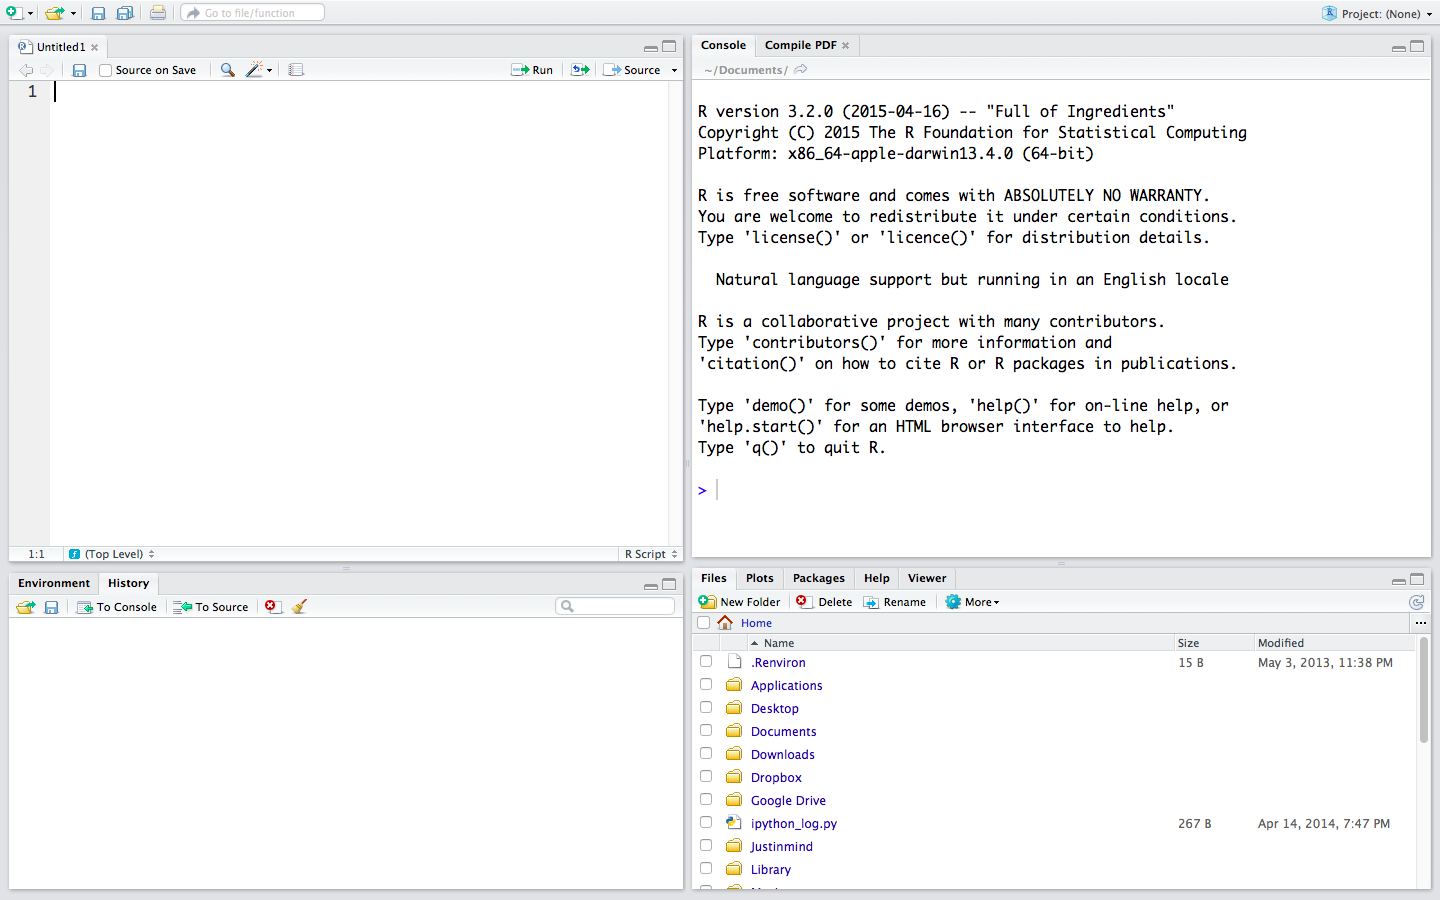
\includegraphics[width=11cm]{images/r-studio.png}
\end{center}

\end{frame}

%------------------------------------------------

\begin{frame}
\frametitle{RStudio}

\begin{center}
\Huge R $\neq$ RStudio
\end{center}

\end{frame}

%------------------------------------------------

\begin{frame}
\frametitle{Working with RStudio}

RStudio provides an IDE that makes it really easy to work with R (everything in a single window)

\bi
  \item console pane
  \item source pane
  \item environment \& history pane
  \item files, plots, and help pane
\ei

\end{frame}

%------------------------------------------------

\begin{frame}[fragile]
\frametitle{Working with RStudio}

Create a new R script and type the following commands:
\begin{knitrout}\footnotesize
\definecolor{shadecolor}{rgb}{0.969, 0.969, 0.969}\color{fgcolor}\begin{kframe}
\begin{alltt}
\hlcom{# amount}
\hlstd{units} \hlkwb{<-} \hlnum{3}
\hlstd{price} \hlkwb{<-} \hlnum{2.57}
\hlstd{amount} \hlkwb{<-} \hlstd{units} \hlopt{*} \hlstd{price}

\hlkwd{paste}\hlstd{(}\hlstr{"The total amount is"}\hlstd{, amount)}
\end{alltt}
\end{kframe}
\end{knitrout}

Find out how to run the commands from the script (don't type in the console!)

\end{frame}

%------------------------------------------------

\begin{frame}[fragile]
\frametitle{Working with RStudio}

A simple bar-chart
\begin{knitrout}\footnotesize
\definecolor{shadecolor}{rgb}{0.969, 0.969, 0.969}\color{fgcolor}\begin{kframe}
\begin{alltt}
\hlcom{# amount}
\hlstd{fruits} \hlkwb{<-} \hlkwd{c}\hlstd{(}\hlstr{'apple'}\hlstd{,} \hlstr{'orange'}\hlstd{,} \hlstr{'peach'}\hlstd{)}
\hlstd{units} \hlkwb{<-} \hlkwd{c}\hlstd{(}\hlnum{5}\hlstd{,} \hlnum{7}\hlstd{,} \hlnum{3}\hlstd{)}
\hlstd{price} \hlkwb{<-} \hlkwd{c}\hlstd{(}\hlnum{0.8}\hlstd{,} \hlnum{0.5}\hlstd{,} \hlnum{0.6}\hlstd{)}
\hlstd{amount} \hlkwb{<-} \hlstd{units} \hlopt{*} \hlstd{price}
\hlkwd{barplot}\hlstd{(amount,} \hlkwc{names.arg} \hlstd{= fruits)}
\end{alltt}
\end{kframe}
\end{knitrout}

What things can you do in RStudio with a plot?

\end{frame}

%------------------------------------------------

\begin{frame}
\frametitle{Working with RStudio}
Menu buttons of an RStudio script
\begin{center}
\ig[width=8cm]{images/rscript.png}
\end{center}
\end{frame}

%------------------------------------------------

\begin{frame}
\frametitle{Customize RStudio}

On the menu bar go to \textit{RStudio} and then go to \textit{Preferences}. Customize the following:

\bi
  \item Pane Layout
  \item Appearance: font type, size, and theme
  \item R General
  \item Code Editing
\ei

Also check the RStudio keyboard shortcuts (see \code{Help})

\end{frame}

%------------------------------------------------

\begin{frame}
\frametitle{RStudio Documentation}

In the manu bar click on \code{Help} and then go to \code{RStudio Docs}
\begin{center}
\ig[width=5cm]{images/rstudio-docs.png}
\end{center}
More at \url{https://support.rstudio.com/hc/en-us}

\end{frame}

%------------------------------------------------

\begin{frame}
\frametitle{RStudio Docs}

\begin{center}
\ig[width=10cm]{images/shortcuts.png}
\end{center}
and many more 

\end{frame}

%------------------------------------------------

\begin{frame}
\frametitle{R and RStudio}

\bbi
  \item We use RStudio because it makes many things easier
  \item However, nothing we produce requires RStudio to be created
  \item RStudio is the means, NOT the end
  \item The important thing is R (and its packages)
\ei

\end{frame}

%------------------------------------------------

\begin{frame}
\frametitle{R Packages}

\bbi
  \item Functions in R are structured in packages (a.k.a. \textit{libraries}*)
  \item The basic distribution of R comes with a number of default (pre-installed) packages
  \item e.g. \code{"stats", "utils", "graphics"}, etc.
  \item To be used, most packages need to be loaded via the function \code{library()}
  \item In addition to the default distributed packages, there is an extensive (and growing) list of contributed packages
\ei

\end{frame}

%------------------------------------------------

\begin{frame}[fragile]
\frametitle{Installing Packages}

R comes with some pre-installed packages. However, one of the benefits of R is the availability of external packages. To install a package use the function {\hilit \code{install.packages()}}
\begin{knitrout}\footnotesize
\definecolor{shadecolor}{rgb}{0.969, 0.969, 0.969}\color{fgcolor}\begin{kframe}
\begin{alltt}
\hlkwd{install.packages}\hlstd{(}\hlstr{"knitr"}\hlstd{)}
\end{alltt}
\end{kframe}
\end{knitrout}

\end{frame}

%------------------------------------------------

\begin{frame}[fragile]
\frametitle{Loading Packages}

Once a package is installed, we use the function {\hilit \code{library()}} to actually load the package and be able to use its functions:
\begin{knitrout}\footnotesize
\definecolor{shadecolor}{rgb}{0.969, 0.969, 0.969}\color{fgcolor}\begin{kframe}
\begin{alltt}
\hlkwd{library}\hlstd{(}\hlstr{"knitr"}\hlstd{)}
\end{alltt}
\end{kframe}
\end{knitrout}

\end{frame}

%------------------------------------------------

\begin{frame}[fragile]
\frametitle{Installing Packages}

\bbi
  \item \code{install.packages()} will install R packages in the specified  directory (argument \code{lib}).
  \item If no \code{lib} is specified, R will download packages in your \textbf{Rlibs} directory
  \item In RStudio, you can use the pane with the tab \textbf{packages} to install packages 
\ei

\end{frame}

%------------------------------------------------

\begin{frame}
\begin{center}
\Huge{\hilit{Getting Help}}
\end{center}
\end{frame}

%------------------------------------------------

\begin{frame}[fragile]
\frametitle{Command \code{help()}}

All packages in R provide technical documentation on how to use the available functions. To have access to such documentation we use the function {\hilit \code{help()}}
\begin{knitrout}\footnotesize
\definecolor{shadecolor}{rgb}{0.969, 0.969, 0.969}\color{fgcolor}\begin{kframe}
\begin{alltt}
\hlkwd{help}\hlstd{(vector)}
\end{alltt}
\end{kframe}
\end{knitrout}

Alternatively, we can use the question mark {\hilit \textbf{?}} to ask for the same type of help documentation:
\begin{knitrout}\footnotesize
\definecolor{shadecolor}{rgb}{0.969, 0.969, 0.969}\color{fgcolor}\begin{kframe}
\begin{alltt}
\hlopt{?}\hlstd{vector}
\hlopt{?}\hlstr{"+"}
\hlopt{?}\hlstr{"["}
\end{alltt}
\end{kframe}
\end{knitrout}

\end{frame}

%------------------------------------------------

\begin{frame}[fragile]
\frametitle{Understanding help documentation}

\bi
  \item Function name (and package)
  \item Description
  \item Usage
  \item Arguments
  \item Details, Notes, References
  \item See Also
  \item Examples
\ei

\end{frame}

%------------------------------------------------

\begin{frame}[fragile]
\frametitle{Searching for help}

The use of \code{help()} requires you to know exactly the name of the object you're looking help for. For a more generic search we can use {\hilit \code{help.search()}}, or the shorthand version \code{??}
\begin{knitrout}\footnotesize
\definecolor{shadecolor}{rgb}{0.969, 0.969, 0.969}\color{fgcolor}\begin{kframe}
\begin{alltt}
\hlkwd{help.search}\hlstd{(}\hlstr{"matrix"}\hlstd{)}
\hlopt{??}\hlstd{matrix}
\end{alltt}
\end{kframe}
\end{knitrout}

\code{help.search()} returns a list of functions and packages related with the searched term

\end{frame}

%------------------------------------------------

\begin{frame}[fragile]
\frametitle{Function \code{apropos()}}

A related function is {\hilit \code{apropos}} which returns a list of functions containing the searched term
\begin{knitrout}\footnotesize
\definecolor{shadecolor}{rgb}{0.969, 0.969, 0.969}\color{fgcolor}\begin{kframe}
\begin{alltt}
\hlkwd{apropos}\hlstd{(}\hlstr{"mean"}\hlstd{)}
\end{alltt}
\end{kframe}
\end{knitrout}

\code{help.search()} returns a list of functions and packages related with the searched term

\end{frame}

%------------------------------------------------

\begin{frame}[fragile]
\frametitle{Functions in packages}

To find out about all the functions in a given package, use the \code{help()} function specifying the name of the package you are interested in:
\begin{knitrout}\footnotesize
\definecolor{shadecolor}{rgb}{0.969, 0.969, 0.969}\color{fgcolor}\begin{kframe}
\begin{alltt}
\hlkwd{help}\hlstd{(}\hlkwc{package} \hlstd{=} \hlstr{"graphics"}\hlstd{)}
\end{alltt}
\end{kframe}
\end{knitrout}

\end{frame}

%------------------------------------------------

\begin{frame}[fragile]
\frametitle{Functions in packages}

To get a list of packages contained in your R version, use \code{library()} and specify the \code{lib.loc} argument:
\begin{knitrout}\footnotesize
\definecolor{shadecolor}{rgb}{0.969, 0.969, 0.969}\color{fgcolor}\begin{kframe}
\begin{alltt}
\hlcom{# deafult packages in your R version}
\hlkwd{library}\hlstd{(}\hlkwc{lib.loc} \hlstd{= .Library)}
\end{alltt}
\end{kframe}
\end{knitrout}

\begin{knitrout}\footnotesize
\definecolor{shadecolor}{rgb}{0.969, 0.969, 0.969}\color{fgcolor}\begin{kframe}
\begin{alltt}
\hlcom{# installed R packages in my computer}
\hlkwd{library}\hlstd{(}\hlkwc{lib.loc} \hlstd{=} \hlstr{"/Users/Gaston/Rlibs"}\hlstd{)}
\end{alltt}
\end{kframe}
\end{knitrout}

In RStudio, you can also use the pane with the tab \textbf{packages} to inspect installed packages 

\end{frame}

%------------------------------------------------

\begin{frame}[fragile]
\frametitle{Function in what package?}

To find which package a function belongs, we use the command {\hilit \code{find()}}
\begin{knitrout}\footnotesize
\definecolor{shadecolor}{rgb}{0.969, 0.969, 0.969}\color{fgcolor}\begin{kframe}
\begin{alltt}
\hlkwd{find}\hlstd{(}\hlstr{"t.test"}\hlstd{)}

\hlkwd{find}\hlstd{(}\hlstr{"mean"}\hlstd{)}

\hlkwd{find}\hlstd{(}\hlstr{"boxplot"}\hlstd{)}
\end{alltt}
\end{kframe}
\end{knitrout}

\end{frame}

%------------------------------------------------

\begin{frame}
\frametitle{More resources}

\bi
  \item R website \url{http://www.r-project.org/}
  \item technical manuals \url{http://cran.r-project.org/manuals.html}
  \item Contributed documentation \url{http://www.r-project.org/other-docs.html}
  \item Task Views \url{http://cran.r-project.org/web/views/}
  \item R journal \url{http://journal.r-project.org/}
\ei

\end{frame}

%------------------------------------------------

\begin{frame}
\frametitle{More resources}

Some blogs and groups
\bi
  \item \url{http://www.r-bloggers.com}
  \item \url{http://www.inside-r.org/}
  \item \url{http://www.scoop.it/t/r-for-journalists}
\ei

\end{frame}

%------------------------------------------------

\begin{frame}
\frametitle{More resources}

\bi
  \item lots of youtube videos
  \item {\small \url{http://stackoverflow.com/questions/tagged/r}}
  \item {\small \url{http://stats.stackexchange.com/questions/tagged/r}}
  \item R programming wikibook {\small \url{http://en.wikibooks.org/wiki/R_Programming}}
  \item Quick-R  {\small\url{http://www.statmethods.net/index.html}}
  \item Google
\ei

\end{frame}

%------------------------------------------------

\begin{frame}
\frametitle{Getting Started}

\bi
  \item \textbf{R for Beginners} by Emmanuel Paradis \\
  \url{http://cran.r-project.org/doc/contrib/Paradis-rdebuts_en.pdf}
  \item {\small \url{http://stats.stackexchange.com/questions/tagged/r}}
  \item R programming wikibook {\small \url{http://en.wikibooks.org/wiki/R_Programming}}
  \item Quick-R  {\small\url{http://www.statmethods.net/index.html}}
  \item Google
\ei

\end{frame}

%------------------------------------------------


\end{document}
